\section{问题二:基于学院打分特点的教师教学评分重计算模型构建}


\subsection{问题重述}

随着2024年该校将教师课堂教学评价任务下放至各学院自行组织,尽管此举旨在提升效率,但也随之带来了评分标准异质性、量尺使用偏差以及内部评价过程可能存在的系统性偏差等一系列挑战。具体表现为学院间评分区间差异显著、得分分布特性不一,以及部分学院内部评分机制可能引入局部偏差,这些因素均可能影响教师教学质量评价的客观性与公平性。本文需分析:

\begin{enumerate}
    \item 如何深入分析附件2中各学院的教学评分数据,识别并量化其在评分标准、打分范围和内部一致性等方面的特点与规律?
    \item 如何提出并建立一个合理的数学模型,以有效消除或减少因学院间差异带来的偏差,对所有教师的教学评分进行重新计算与校准?
    \item 如何对经过模型重新计算后的教师教学评分结果的公平性、有效性及合理性进行全面阐释?
\end{enumerate}

\subsection{Results}

The results of the prediction are shown in the following table.

\begin{figure}[H]
    \centering
    \begin{minipage}[t]{0.32\textwidth}
        \centering
        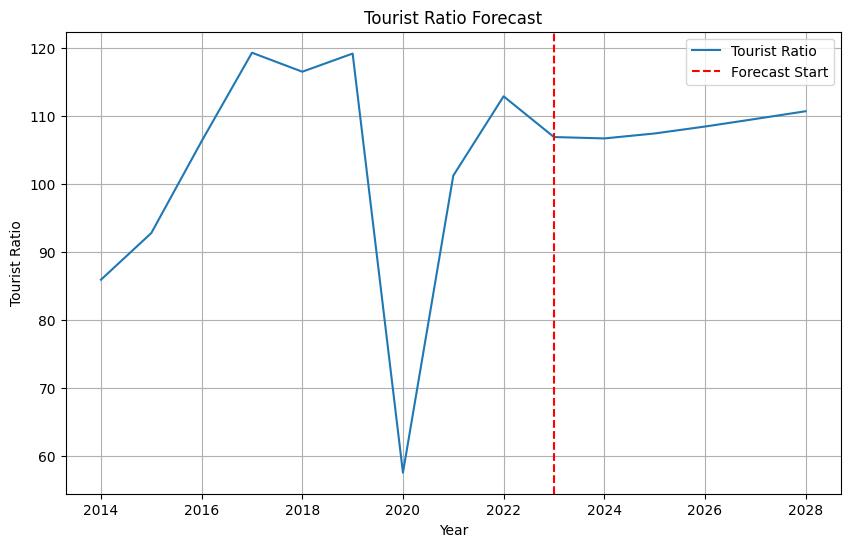
\includegraphics[width=1\textwidth]{Ratio_Sitka.png}
    \end{minipage}
    \hfill
    \begin{minipage}[t]{0.32\textwidth}
        \centering
        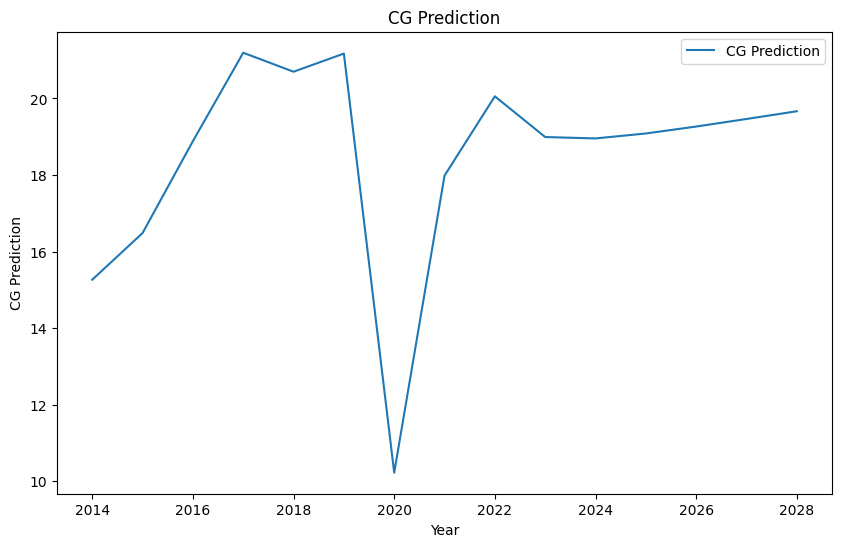
\includegraphics[width=1\textwidth]{CG_Sitka.png}
    \end{minipage}
    \hfill
    \begin{minipage}[t]{0.32\textwidth}
        \centering
        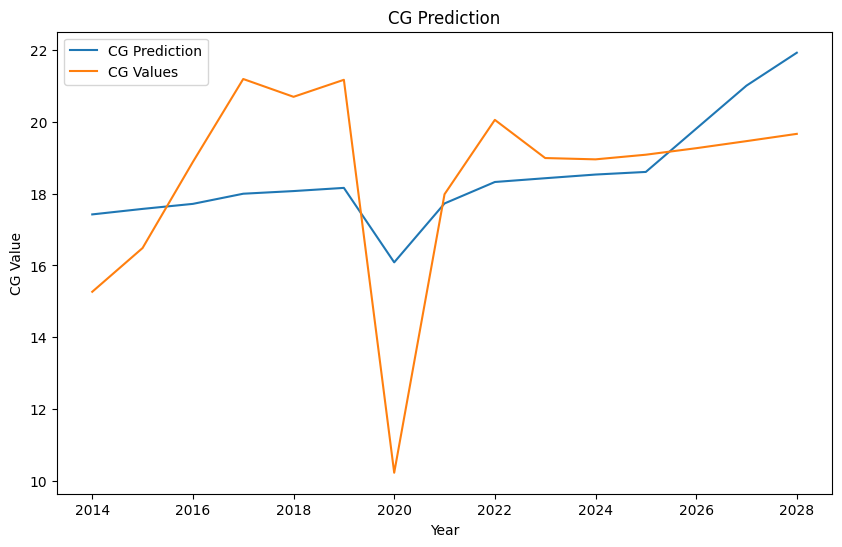
\includegraphics[width=1\textwidth]{CG_Pred_Sitka.png}
    \end{minipage}
\end{figure}

\begin{figure}[H]
    \centering
    \begin{minipage}[t]{0.32\textwidth}
        \centering
        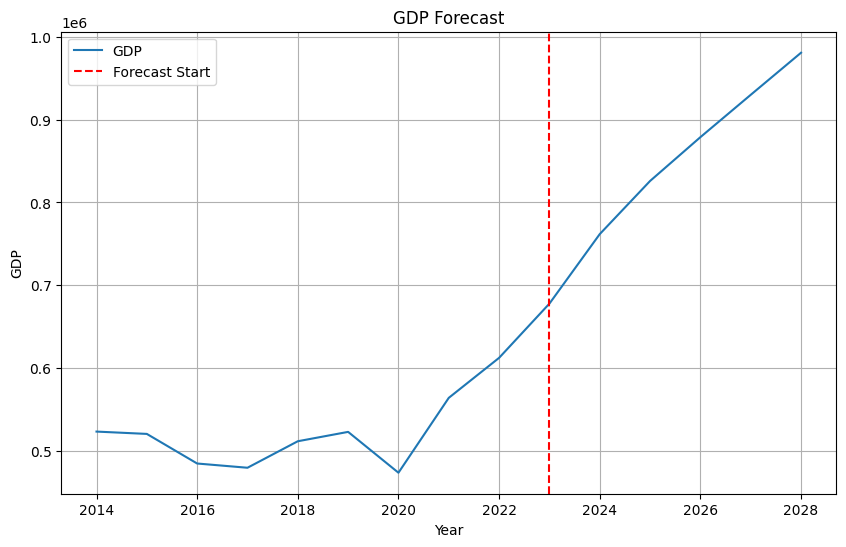
\includegraphics[width=1\textwidth]{GDP_Sitka.png}
    \end{minipage}
    \hfill
    \begin{minipage}[t]{0.32\textwidth}
        \centering
        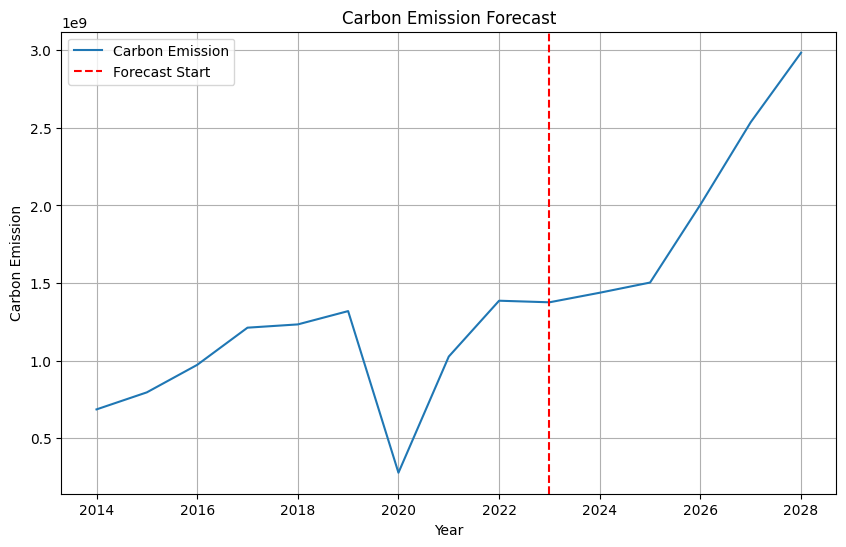
\includegraphics[width=1\textwidth]{C_Emission_Sitka.png}
    \end{minipage}
    \hfill
    \begin{minipage}[t]{0.32\textwidth}
        \centering
        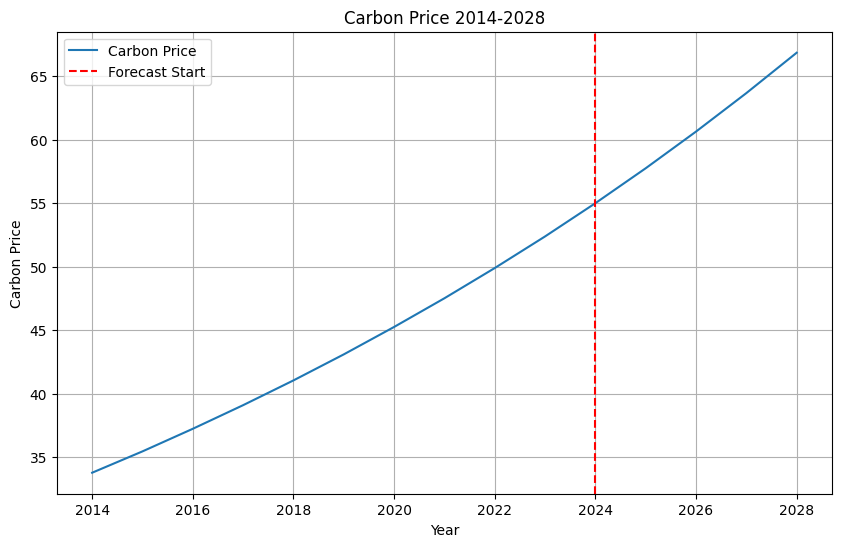
\includegraphics[width=1\textwidth]{C_Price_Sitka.png}
    \end{minipage}
\end{figure}



\begin{figure}[H]
    \centering
    \begin{minipage}[t]{0.5\textwidth}
        \centering
        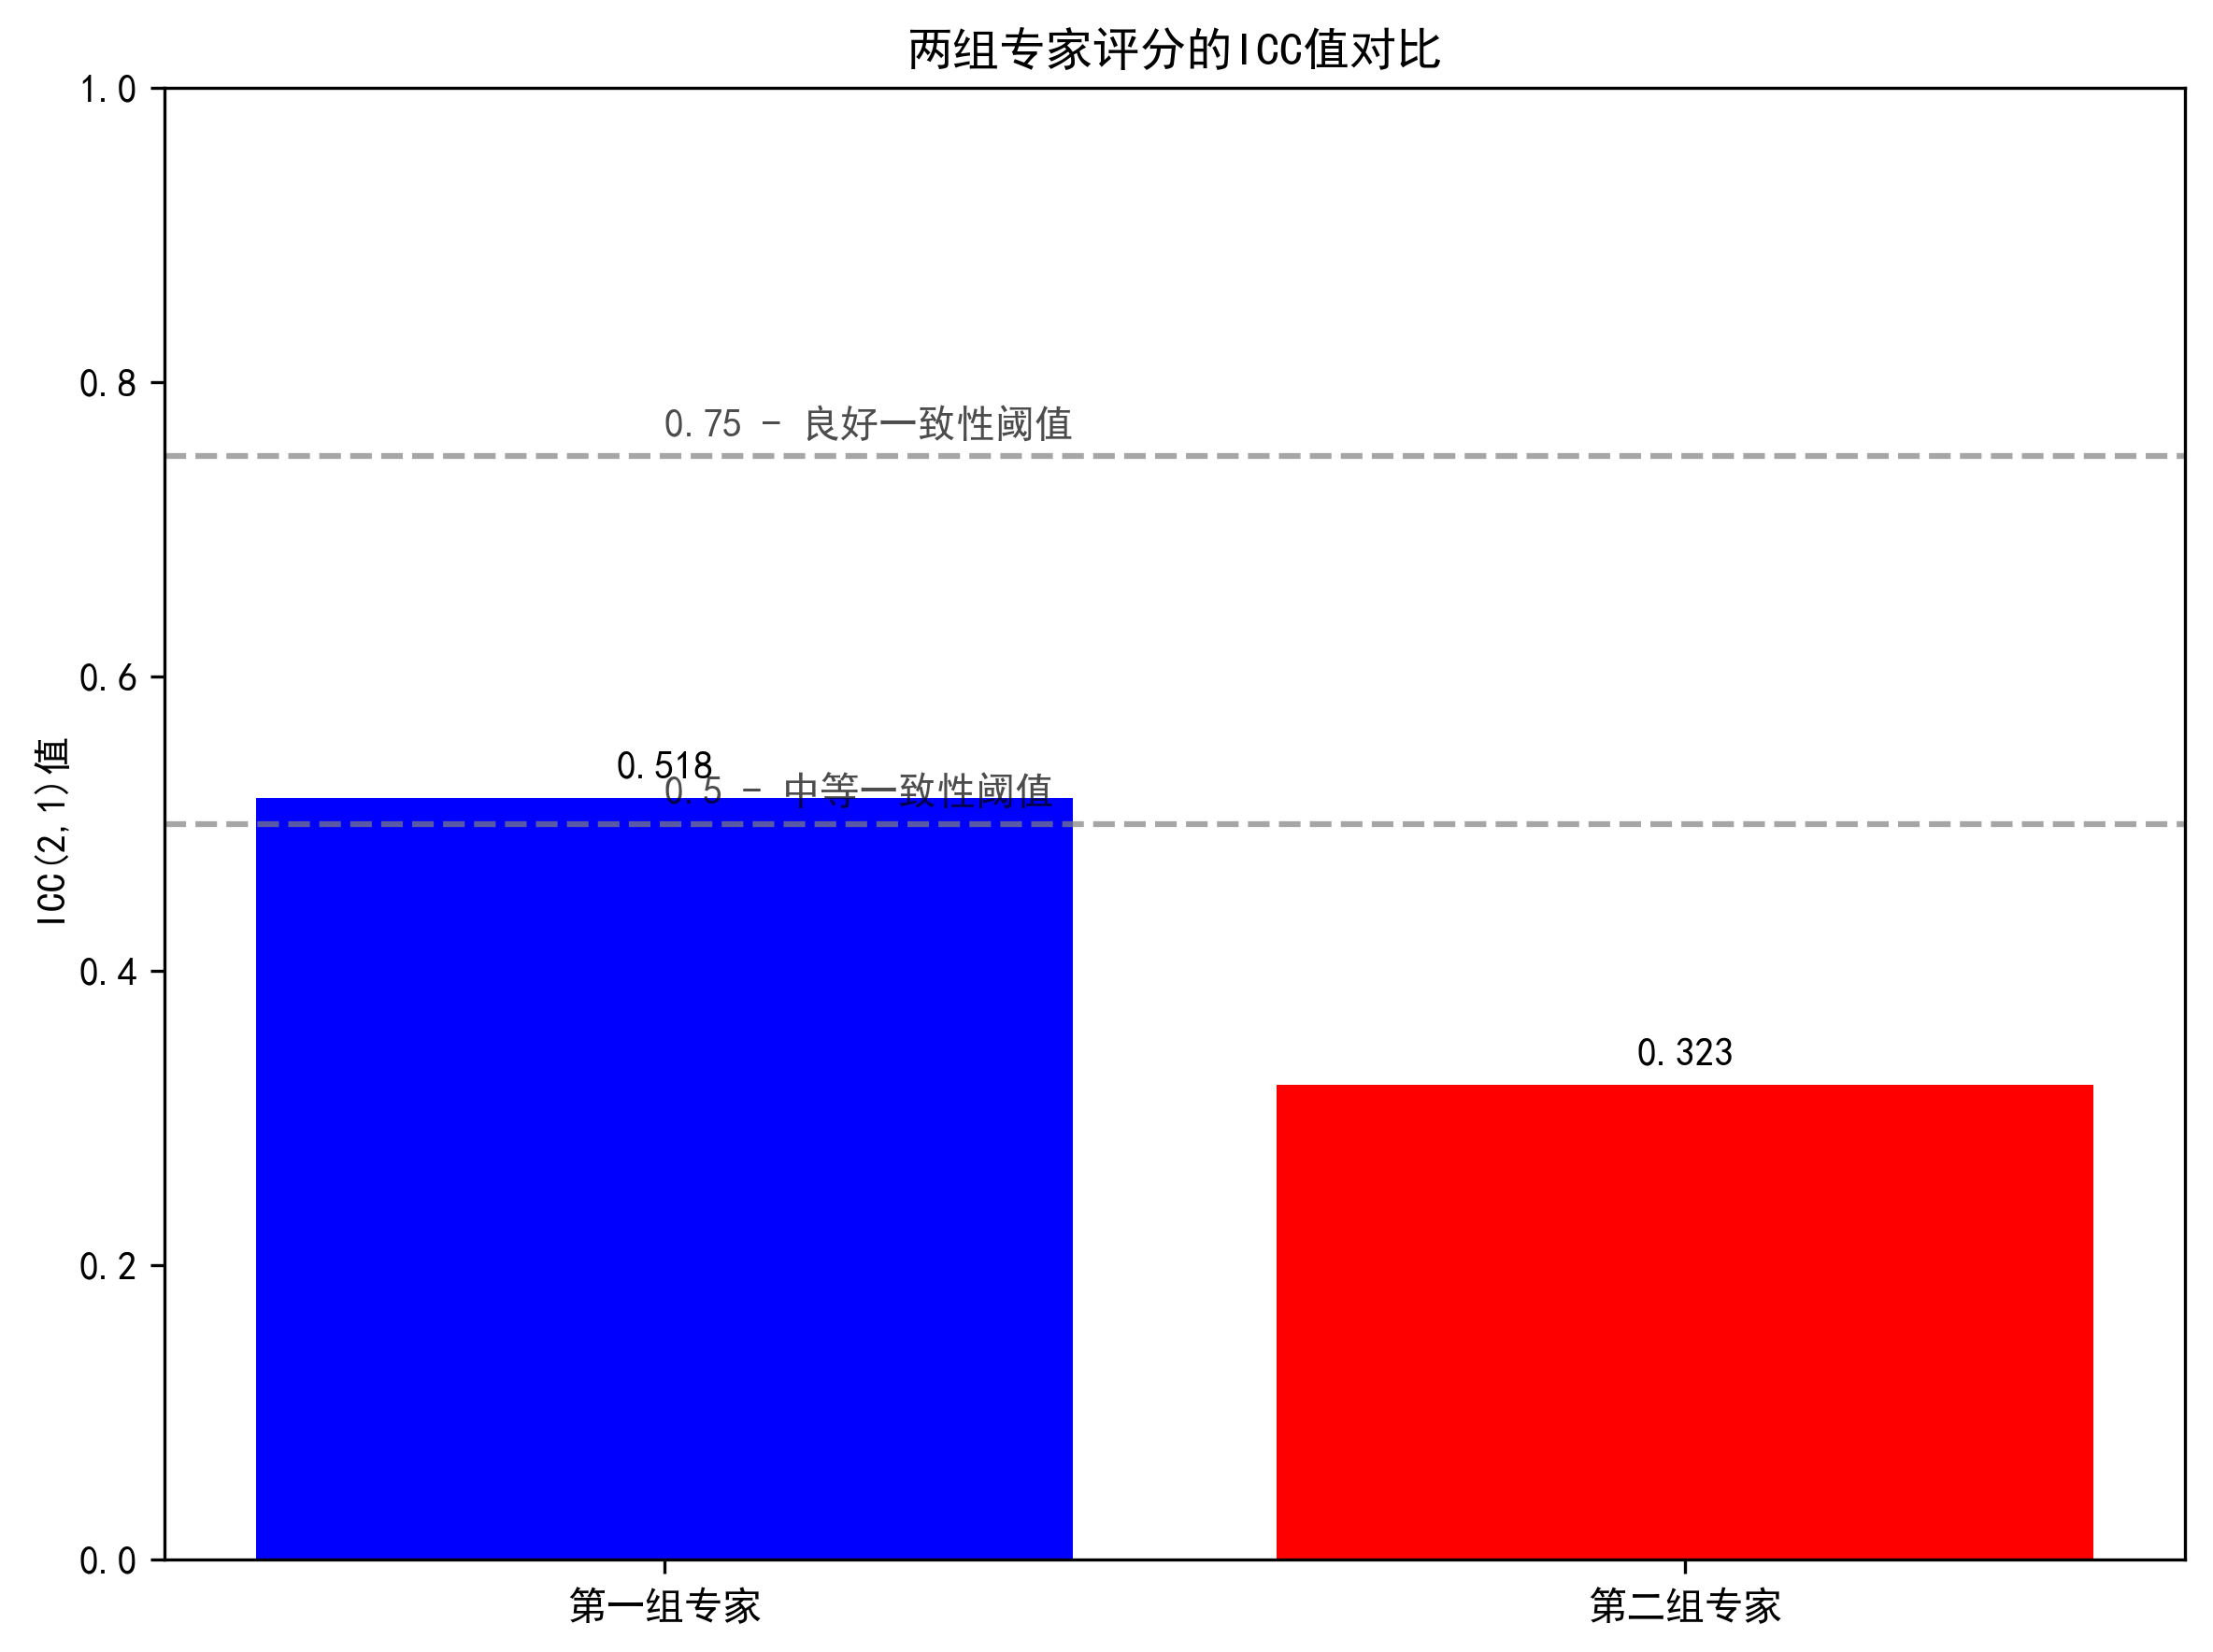
\includegraphics[width=1\textwidth]{icc_analysis.png}
    \end{minipage}
    \hfill
    \begin{minipage}[t]{1\textwidth}
        \centering
        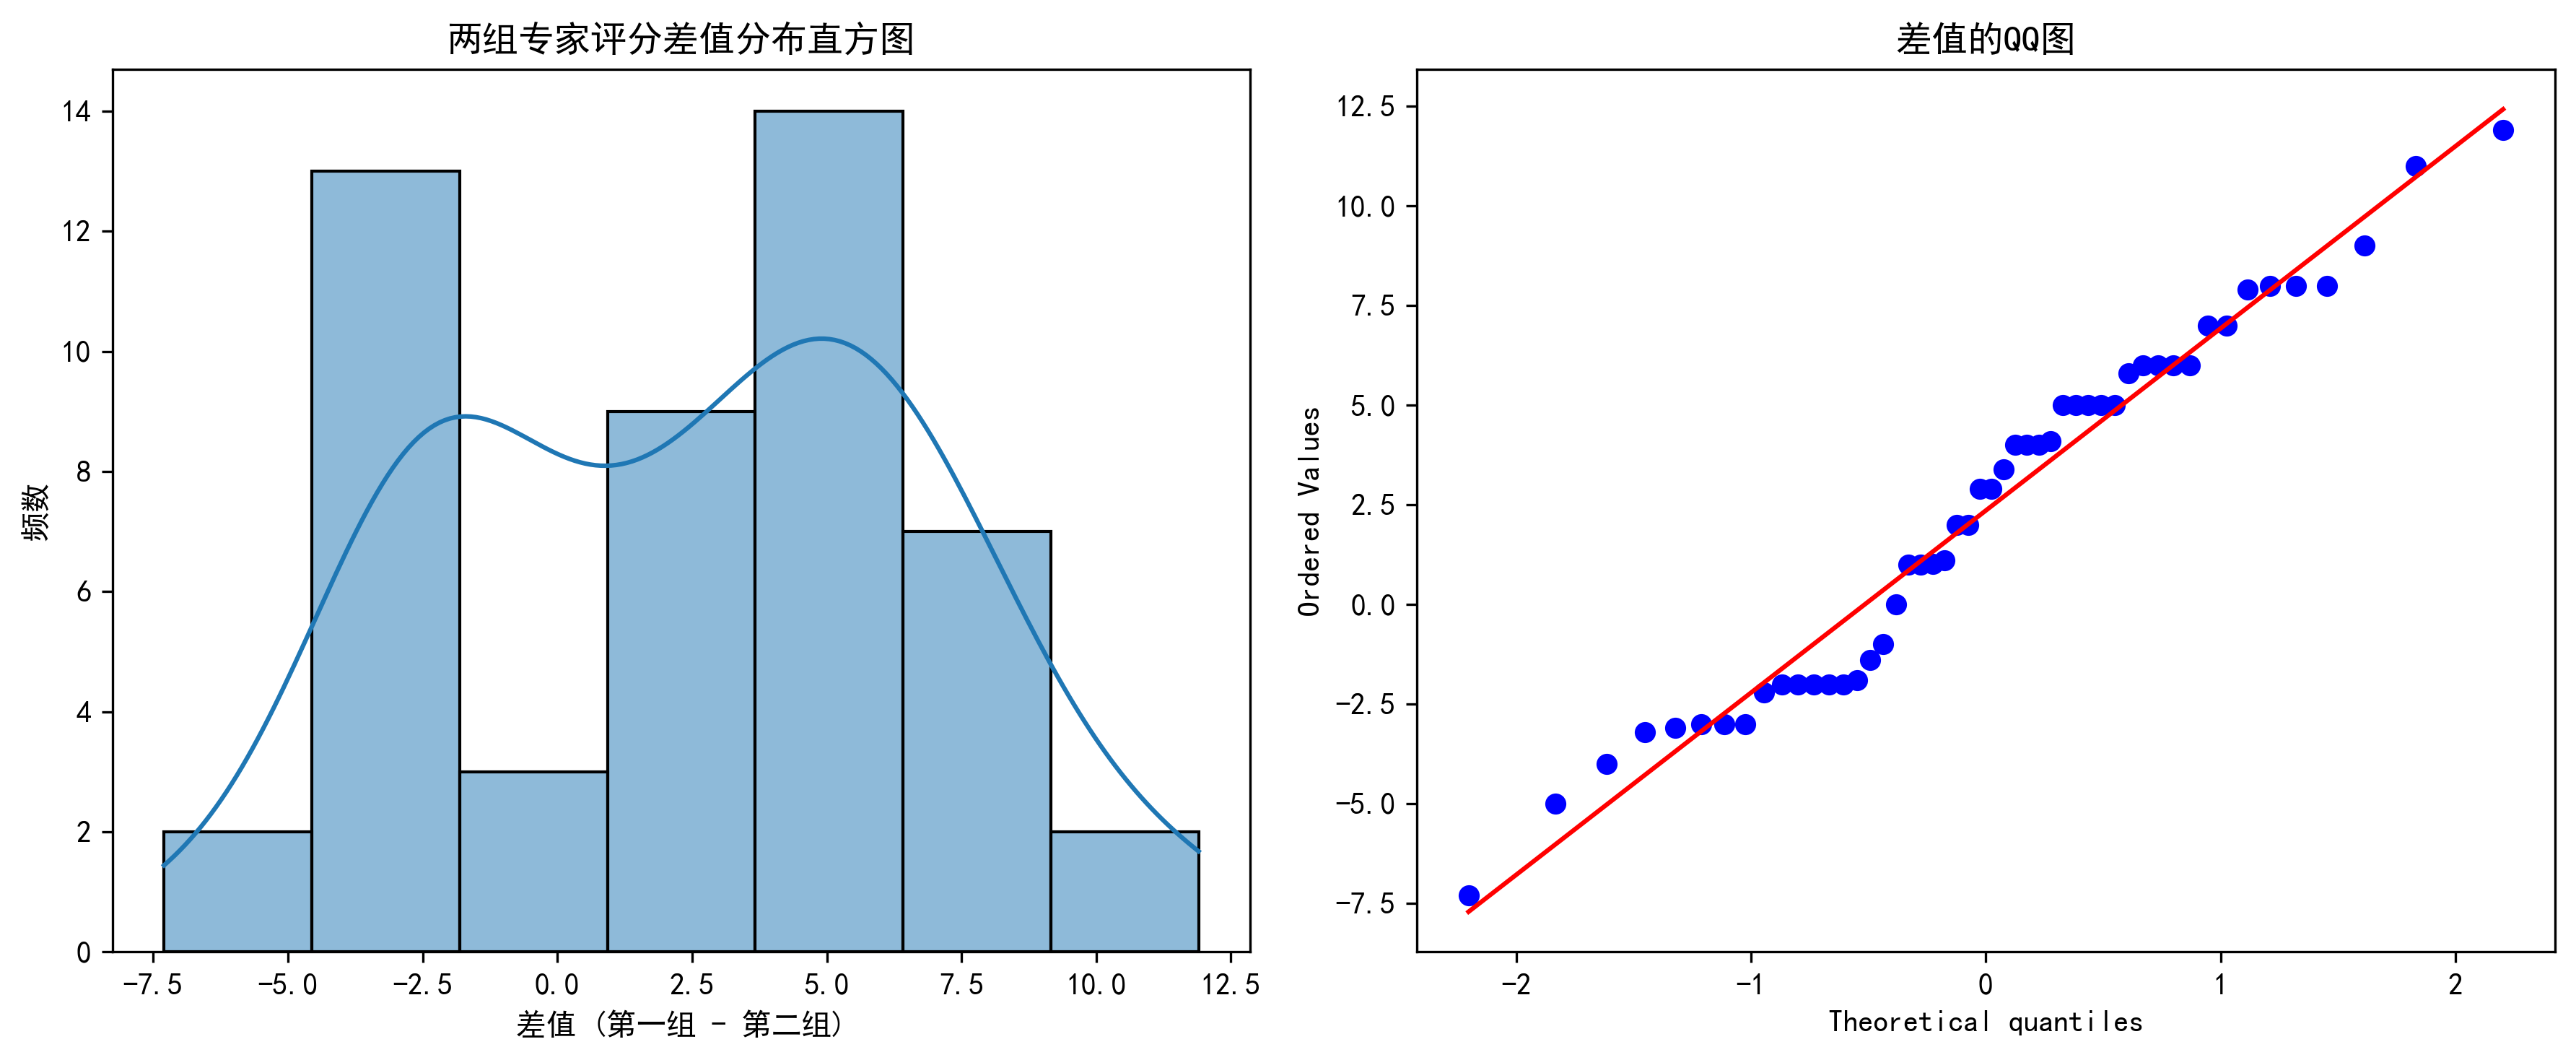
\includegraphics[width=1\textwidth]{normality_test.png}
    \end{minipage}
\end{figure}

\subsection{Analyses}

Summing up all the categories and the parameters yields the final equation.

\begin{equation}
    \begin{aligned}
    &\left\{\begin{array}{l}
    \mathcal{F}=(\alpha \cdot \text { Economy }-\beta \cdot \text { Environment }) / \text { Society } \\[10pt]
    \text { Economy }=165 N \cdot f(\eta) \cdot (\eta+1)+NQ\cdot e^{-0.2 Q} \\[10pt]
    \text { Environment }=2.897 \cdot N^2+ 7.67\times 10^5 N- 3.293\times 10^{10} \\[10pt]
    \text { Society }=5.011\times 10^{-9} N + 4.2 \\[10pt]
    f(\eta)=-5.5 \eta^3+9.1903 \eta^2-5.1903 \eta+1.5, \quad 0 \leq \eta \leq 1
    \end{array}\right.
    \end{aligned}
\end{equation}

When $\alpha$ is set to 1 and $\beta$ is set to 30, 
the optimal value of $N,Q,\eta$ is calculated as follows:

\begin{equation}
    \begin{aligned}
    &\left\{\begin{array}{l}
    N_{Max} = 93.353 \\[10pt]
    N_{LastYear} = 95.937 \\[10pt]
    N=52.04 \\[10pt]
    Q=4.89 \\[10pt]
    \eta=0.286
    \end{array}\right.
    \end{aligned}
\end{equation}

The strategy is the same as we have proposed in Juneau, 
that is to increase the tax rate and the fine rate, and to 
decrease the number of tourists. Thus our model can be successfully
adapted to Sitka, Alaska, proving its adaptability and migration capability.

\subsection{Sensitivity Analysis}

To evaluate the robustness of the migrated model, we conduct a sensitivity analysis.

The results are shown below:

\begin{figure}[H]
    \centering
    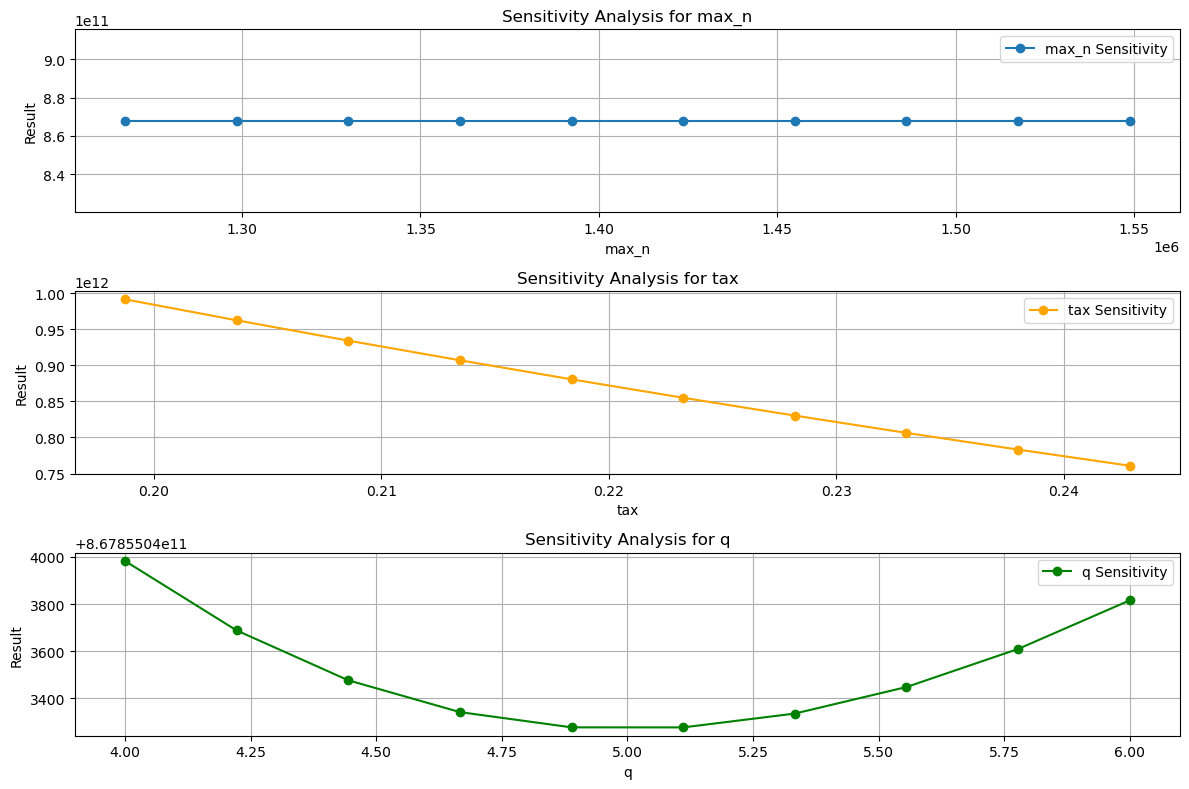
\includegraphics[width=1\textwidth]{Sensitivity_Analysis_Sitka.jpg} % 插入图片
    \vspace{-0.5cm}
    \caption{Sensitivity Analysis}
\end{figure}

It can be shown that when $N_{Max}$ is the independent variable, the outcome is immune to the change of $N_{Max}$,
while in other circumstances are sensitive to the changing of the independent variables.
The result is similar to what we conducted in Juneau.